\documentclass[t]{beamer}

%bibliography
%\usepackage[notes,backend=bibtex,isbn=false,doi=false,eprint=false, note=false, url=false]{biblatex-chicago}
\usepackage[authordate-trad,backend=biber,isbn=false,doi=false,eprint=false, url=false]{biblatex-chicago}
\bibliography{narrative}

% customizing the title page
\defbeamertemplate*{title page}{customized}[1][]
{
  \vspace{1cm}
  \usebeamerfont{title}\inserttitle\par
  \usebeamerfont{subtitle}\usebeamercolor[fg]{subtitle}\insertsubtitle\par
  \vspace{4.5cm}
  \usebeamerfont{date}\insertdate\par
  \vspace{.5cm}
  \usebeamerfont{author}\insertauthor\par
  \usebeamerfont{institute}\insertinstitute\par
  
  
  \usebeamercolor[fg]{titlegraphic}\inserttitlegraphic
}

\usepackage{graphicx}
\usetheme[compress]{Dresden}
\usecolortheme{dove}
\usefonttheme{serif}
%\usefonttheme{structureitalicserif}
%\usepackage{helvet}
%\usefonttheme{professionalfonts}
%gets rid of bottom navigation bars
\setbeamertemplate{footline}[frame number]{}
\usepackage[utf8]{inputenc}
\usepackage[norsk]{babel}
\usepackage{appendix}
\usepackage[export]{adjustbox}
\usepackage{wrapfig}
\setbeamertemplate{caption}{\insertcaption}
\usepackage{tikz}
\usepackage{multirow} % to have tables with rows over multiple lines


\title{\huge Topic modeling}
\subtitle{A brief (semi-technical) walk through the algorithm)}
%\vspace{6cm} % this doesn't seem to do anything...
\author{Gregory Ferguson-Cradler}
\institute{Institutt for rettsvitenskap, filosofi og internasjonale studier \\ Høgskolen i Innlandet, Lillehammer}
\date{NTNU, Trondheim, 12.-13. August 2021} %\today}
 
% \AtBeginSubsection[]
% {
% \begin{frame}<beamer>{Overview}
% \tableofcontents[currentsection, currentsubsection, currentsubsubsection,
%     %hideothersubsections, 
%     sectionstyle=show/shaded,
% ]
% \end{frame}
% }
 
\begin{document}

\begin{frame}[plain]
    \titlepage    
\end{frame}

% \begin{frame}[plain]%{1944}
% %\frametitle{\vspace{-.5cm}Frame Title Goes Here}
% \begin{figure}
% %\vspace*{-.5cm}
% \includegraphics[width=1\textwidth, valign=c]{Frontene.jpg} 
% %\caption{Frontene i Europa i 1944}
% \end{figure}
% \end{frame}

\begin{frame}{The assumptions behind the topic model algorithm}
\begin{figure}
    \centering
    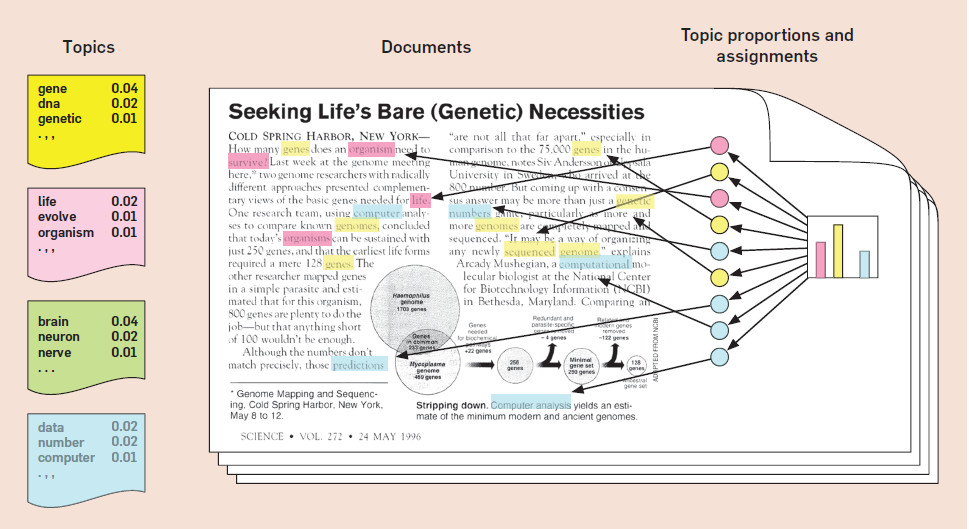
\includegraphics[width=.9\linewidth]{blei.jpg}
    \caption{Text is produced by chosing a distribtion of topics within the given document; the for every word a selection of topic based on the document-level distribution; finally a word from the corresponding topic \autocite[78]{blei2012probabilistic}.}
    \label{fig:Blei}
\end{figure}
\end{frame}

\begin{frame}{The document generating process}
\begin{figure}
    \centering
    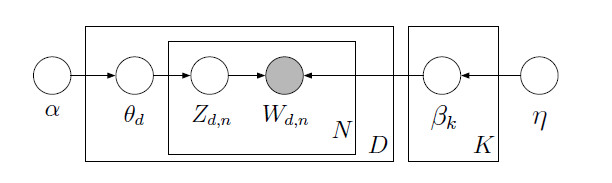
\includegraphics[width=.8\linewidth]{blei2.jpg}
    \caption{Interrelations of the probabalistic data generating process \autocite[78]{blei2009topic}.}
    \label{fig:Blei}
\end{figure}

\begin{itemize}[<+->]
    \item $\vec{\beta}_{k} \sim \text{Dir}_V(\eta)$
    \item $\vec{\theta}_{d} \sim \text{Dir}_k (\vec{\alpha})$
    \item $Z_{d,n} \sim \text{Mult}(\vec{\theta}), Z_{d,n} \in \{1,...,K\}$
    \item $W_{d,n} \sim \text{Mult}(\vec{\beta}_{Z_{d,n}}), W_{d,n} \in \{1,...,V\}$
\end{itemize}
\end{frame}

\begin{frame}{Fitting the model}

First, randomly assign a topic to each word in the document. We can now compute $\theta$ and $\beta$ distributions. Now, for every word, compute:
$$ P(K|d,n) = \frac{tf_{K,n} + \eta}{tf_K} \cdot (tf_{K,d} + \alpha)$$
and reassign based on new most likely topic assignment.

\begin{itemize}[<+->]
    \item This is a process that does not seem much like the act of writing as we know it, but it \textit{might} give interesting results.
    \item One parameter we must set: k. Best practices recommend fiddling with it until you get a model fit that is coherent.
    \item Concentration hyperparameters ($\eta$ and $\alpha$) -- the higher they are the more even $\beta$ and $\theta$. 
    \item Our two matrices of interest: $\theta$ and $\beta$.
\end{itemize}
\end{frame}

\begin{frame}{Practice}
\vspace*{\fill}
\centering Enough Greek letters, let's see how to do this in practice.
\vspace*{\fill}
\end{frame}

\end{document}

